	\begin{figure}[H]
		\centering
 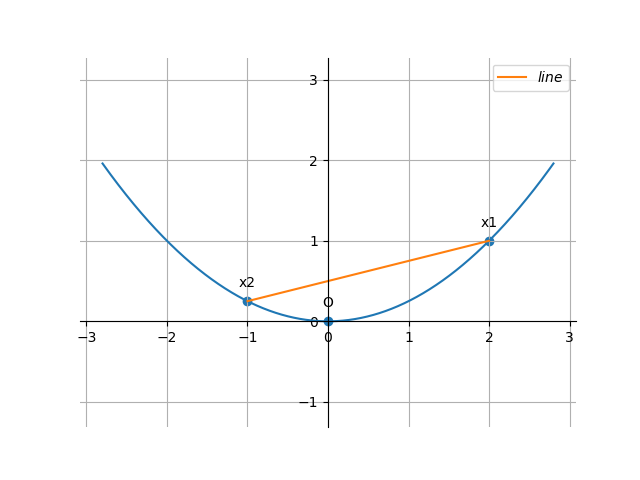
\includegraphics[width=0.75\columnwidth]{chapters/12/8/1/10/figs/conic.png}
		\caption{}
		\label{fig:12/8/1/10}
  	\end{figure}
The given curve  can be expressed as a conic with parameters
\begin{align}
	\vec{V} &= \myvec{1 & 0\\0 & 0}, \vec{u} = \myvec{0 \\-2}, f = 0
	\end{align}
The parameters of the given line are
\begin{align}
\vec{q} = \myvec{-2 \\0} , \vec{m}=\myvec{4\\1}
\end{align}
The points of intersection can then be obtained from \eqref{eq:tangent_roots} 
\begin{align}
\therefore \vec{x}_1=\myvec{2\\1} , \vec{x}_2=\myvec{-1\\ \frac{1}{4}}
\end{align}
The desired area is then obtained 
from 		\figref{fig:12/8/1/10}
as
\begin{align}
	A&=\int_{x_2}^{x_1} [f(x)-g(x)] \,dx
	\\
	&=\int_{-1}^{2} \brak{\frac{x+2}{4}-\frac{x^2}{4}} \,dx
	\\
	& = \frac{9}{8} 
\end{align}
